%***** Preamble *****%
\documentclass[a4paper]{article}

%% Language and font encodings
\usepackage[english]{babel}
\usepackage[utf8x]{inputenc}
\usepackage[T1]{fontenc}

%% Sets page size and margins
\usepackage[a4paper,top=3cm,bottom=2cm,left=3cm,right=3cm,marginparwidth=1.75cm]{geometry}

%% Useful packages
\usepackage{amsmath}
\usepackage{graphicx}
\usepackage[colorinlistoftodos]{todonotes}
\usepackage[colorlinks=true, allcolors=blue]{hyperref}

\usepackage{float} % Usado para posicionar imagens
\usepackage{enumitem} % Usado para criar listas enumeradas com letras
\usepackage{caption} % Adiciona comandos aos captions de figures

\title{Curso de Verilog - Dia 2}
\author{Caio Rodrigo, Jorge Reis}
\date{} % No Date
%%%%%%%%%%%%%%%%%%%%%%%%%%%%%%%%%%%%%%%%%%%%%%%%%%%%%%%%%%%%%%%%%
%***** Document *****%
\begin{document}
\maketitle

%***** Prática 3 - Testbenches *****%
\section*{Prática 3 - Testbenches}

\subsection*{Atividades}
Crie um testbench para cada um dos dois módulos propostos na aula passada: Mux 2x1 e Full Adder. Verifique se os módulos estão funcionando corretamente.

%****** Prática 4 - Dataflow *****%
\section*{Prática 4 - Dataflow}

\subsection*{Atividades}
Utilize modelagem em nível de dataflow para resolva as questões abaixo. Você pode usar o testbench da prática anterior em cada módulo.

\begin{enumerate}
\item Construa os circuitos abaixo. \textbf{Restrição}: não utilize o operador ternário "?:" para o multiplexador e o operador "+" para o somador.
	\begin{figure}[H]
	\centering
	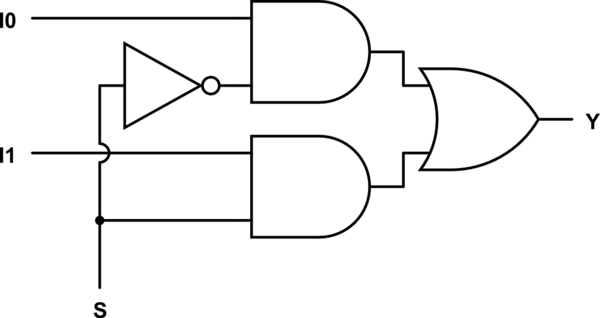
\includegraphics[width=0.3\textwidth]{images/mux2x1.jpg}
    \caption*{Multiplexador 2x1}
	\end{figure}
    
    \begin{figure}[!h]
	\centering
	
\includegraphics[width=0.3\textwidth]{images/fulladder.jpg}
    \caption*{Full Adder}
	\end{figure}
		
\item Construa um módulo \textbf{ALU} que receba como entrada dois valores (a e b) de 4 bits e uma entrada de seleção (s) de 2 bits. O módulo deverá possuir uma saída (c) de 8 bits e produzir o resultado de acordo com a operação escolhida pela entrada de seleção da seguinte forma:
	\setlist[enumerate,1]{start=0} % only outer nesting level
	\begin{itemize}
		\item s = 2'b00; add;
		\item s = 2'b01; sub;
		\item s = 2'b10; mul;
		\item s = 2'b11; div;
	\end{itemize}
\end{enumerate}

Verifique a funcionalidade do módulo por meio de um testbench.

\end{document}